% \vspace{5mm}
\section{Datasets\label{datasets}}
In this section, different datasets used in various pre-training tasks and ablation study for \cite{wang-etal-2022-lilt} is described. All the models have an equal amount of self-attention layers, attention heads and maximum sequence length in order to make sure that BiACM can work normally. The \text{BASE}  setting contains 12-layer encoder with 192 hidden layers, 768 feed-forward filter size and 12 attention heads. The resulting parameters is 6.1M and the maximum sequence length N is 512. Adam Optimizer (Adaptive Moment Estimation) \cite{loshchilov2017decoupled} was used with the learning rate of $2\times10^{-5}$, this optimizer helps to reduce the loss while training the neural networks.



\subsection{IIT-CDIP}
IIT-CDIP \cite{lewis2006building} was build with the aim of achiving \acrfull{cdip} and support different component technologies like document structure analysis, optical character recognition, signature and logo recognition, authorship attribution, named entity recognition and so on. The dataset is based on a collection of roughly 40 million scanned images from the Legacy Tobacco Documents Library \cite{schmidt2002building}. An example of a document from the dataset is shown in \Cref{fig:IIT-CDIP} indicating document image, some portions of its metadata and a few words derived from OCR. The documents shows some of difficult challenges for processing a complex document such as multiple fonts, poor reproduction quality and information in handwritten annotations.  

\begin{figure}[ht]
    \centering
    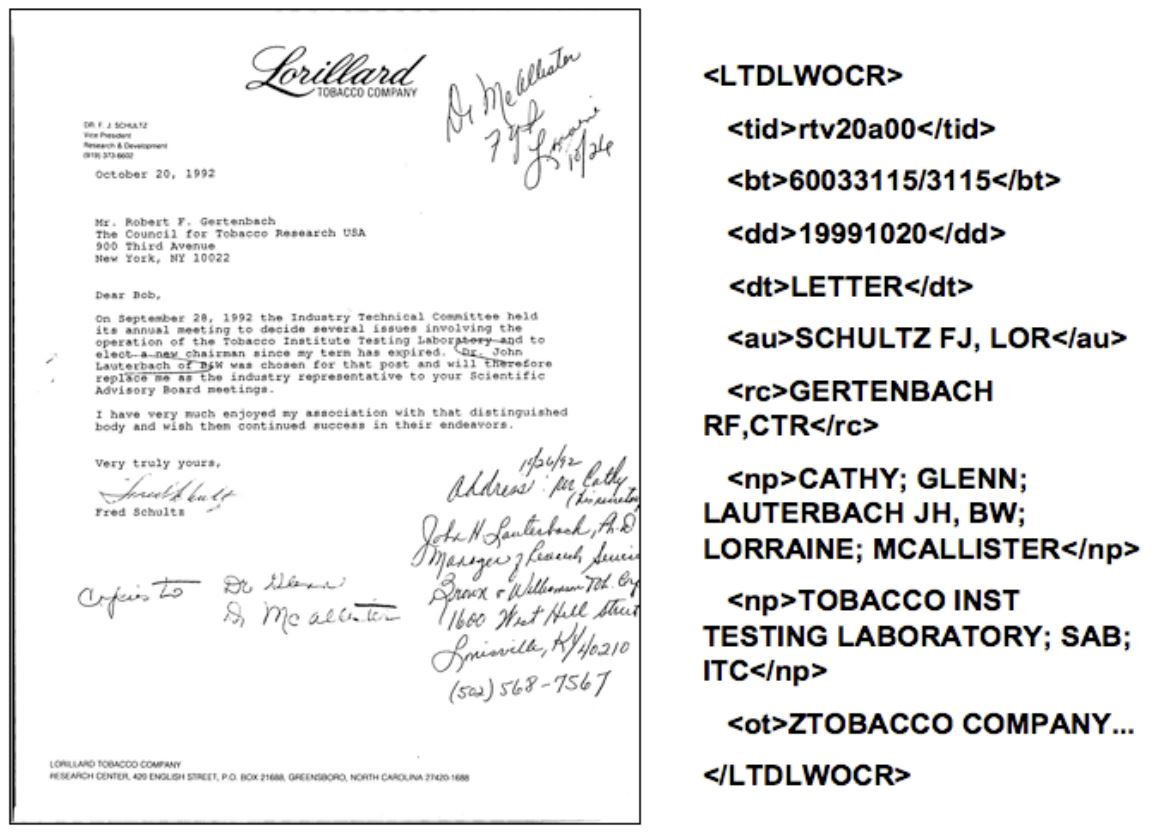
\includegraphics[width=0.7 \textwidth]{chapters/images/Methods/Datasets/IIT-CDIP.JPG}
    \caption{An example document from IIT-CDIP \cite{lewis2006building}}
    \label{fig:IIT-CDIP}
\end{figure}


In the pre-training of \acrshort{lilt}, the RVL-CDIP \cite{lewis2006building} dataset was used. The dataset is a subset of IIT-CDIP prepared by \cite{harley2015evaluation}. RVL-CDIP contains 400,000 gray-scale images of English documents, the images are categorized into 16 different classes. The existing pre-trained English \(RoBERTa_{BASE}\) \cite{liu2019roberta} was used in combination with LiLT\(_{BASE}\) to pre-train the model for document understandig in one language, which will be replaced to multilingual pre-trained InfoXLM\(_{BASE}\) \cite{chi2020infoxlm} for fine-tunning in order to make the overall model multilingual.  With the batch size of 96, LiLT\(_{BASE}\) was trained for 5 epochs on the RVL-CDIP dataset using 4 NVIDIA A40 48GB GPUs.



\subsection{FUNSD}

FUNSD \cite{jaume2019funsd} is a dataset for form understanding in noisy scanned documents. The aim is to extract and structure the textual content of forms. The dataset is made of 199 real, fully annotated, scanned forms and it can be used for various tasks such as text detenction, \acrlong{ocr}, spatial layout analysis and entity labeling/linking. FUNSD dataset is a subset of the RVL-CDIP\footnote{\url{https://www.cs.cmu.edu/ aharley/rvl-cdip/}, Accessed: 09.04.2024}, which includes 400,000 grayscale images of various documents from the 1980s-1990s. In the process of building FUNSD, 25,000 images were checked from the form categories. Unreadable and similar forms were discareded, resulting in 3,200 documents. Among them 199 documents were randomly sampled to annotate as shown in \Cref{fig:FUNSD_ex}, where different classes like headers, question, answer and others are denoted in yellow, blue, green and violate colours respectively. In \Cref{tab:Class distribution FUNSD}, the class distribution of semantic entities from FUNSD dataset is described. LiLT\(\text{[EN-R]}_{BASE}\) is using existing pre-trained on English language corpus \(\text{RoBERTa}_{BASE}\) \cite{liu2019roberta} in combination with \acrshort{lilt} as shown in \Cref{fig:lilt_framework}. \(\text{LiLT[InfoXLM]}_{BASE}\) is using existing pre-trained in multi language corpus  \(\text{InfoXLM}_{BASE}\) \cite{chi2020infoxlm} in combination with \acrshort{lilt}. In paper \cite{wang-etal-2022-lilt}, authors have compared both [EN-R] and [InfoXLM] pre-trained models with BASE setting using FUNSD \cite{jaume2019funsd} dataset. The evaluation result describe in \Cref{tab:pre-trained_model_comparision} is based on \acrfull{ser} task on FUNSD dataset. According to the \Cref{tab:pre-trained_model_comparision}, we can see that the pre-trained model LiLT\(\text{[EN-R]}_{BASE}\) has higher Precision, Recall and F1 with compare to LiLT\(\text{[InfoXLM]}_{BASE}\) when the model is applied to \acrshort{ser} task on the same dataset.

\begin{figure}[H]
    \centering
    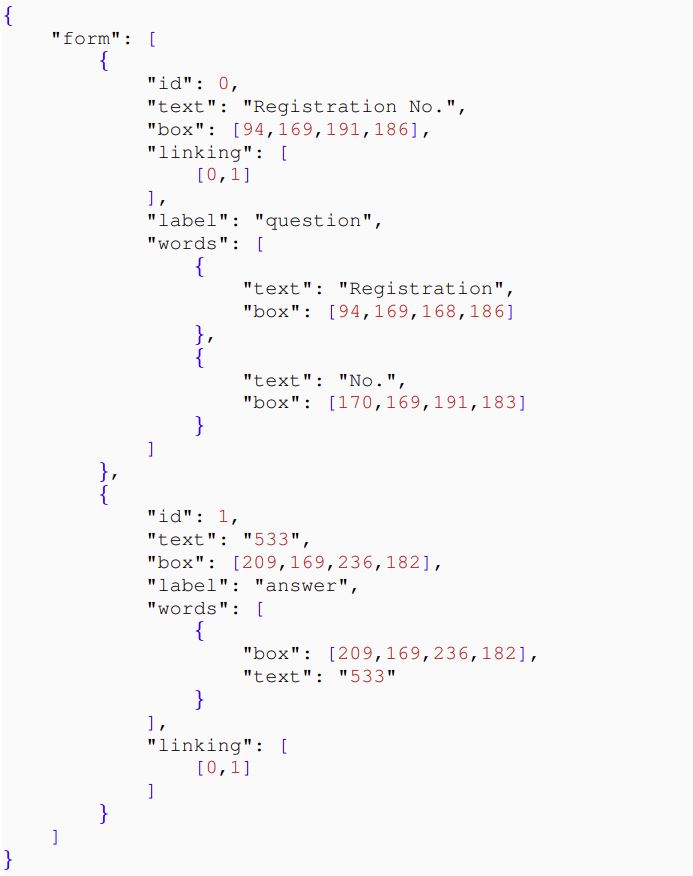
\includegraphics[width=0.5 \textwidth]{chapters/images/Methods/Datasets/FUNSD.JPG}
    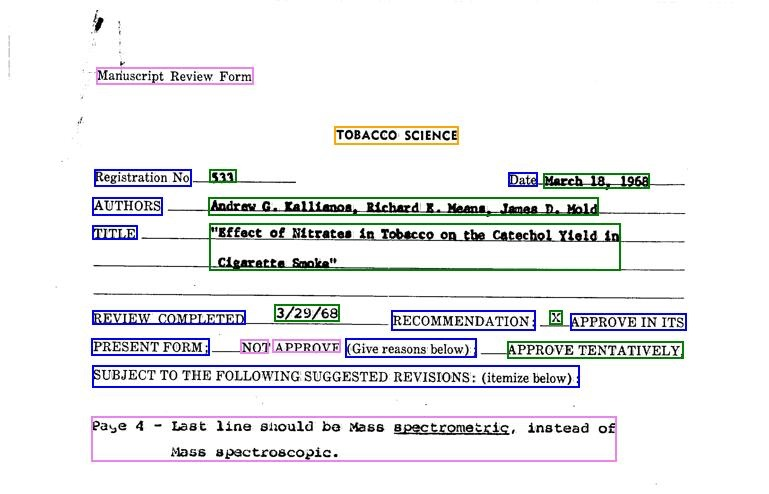
\includegraphics[width=0.8 \textwidth]{chapters/images/Methods/Datasets/different_classes.jpg}
    \caption{An Example of ground-truth format of a document from FUNSD \cite{jaume2019funsd} with different classes}
    \label{fig:FUNSD_ex}
\end{figure}

\begin{table}[H]
    \centering
    \begin{tabular}{lccccl}
    \hline
    \textbf{Split} & \textbf{Header} &\textbf{Question}& \textbf{Answer} & \textbf{Other} & \textbf{Total} \\ \toprule
    Training & 441 & 3,266 & 2,802 & 902 & 7,411 \\
    Testing & 122 & 1,077 & 821 & 312 & 2,322 \\ \bottomrule
    \end{tabular}
    \caption{Class distribution of the semantic entities in FUNSD}
    \label{tab:Class distribution FUNSD}
\end{table}

\begin{table}[H]
    \centering
    \captionsetup{justification=centering}
    \begin{tabular}{lccl}
    \hline
    \textbf{Model}& \textbf{Precision} & \textbf{Recall} & \textbf{F1} \\ \toprule
     RoBERTa\(_{BASE}\)$^1$ & 0.634 & 0.697 &0.664 \\
     LayoutXLM\(_{BASE}\)$^2$ & 0.791 & 0.815 & 0.803 \\
     \hline
     LiLT\(\text{[EN-R$^1$]}_{BASE}\) &  0.872&  0.896& 0.884 \\ 
     LiLT\(\text{[InfoXLM$^3$]}_{BASE}\) & 0.846 & 0.870 & 0.858 \\ \bottomrule
    \end{tabular}
    \caption{Comparision of \acrfull{ser} task on FUNSD \cite{jaume2019funsd} dataset.$^1$\cite{liu2019roberta}, $^2$\cite{xu2021layoutxlm},$^3$\cite{chi2020infoxlm}}
    \label{tab:pre-trained_model_comparision}
\end{table}

The term Precision, Recall and F1 is refers to the confusion matrix \ref{tab:Confusion Matrix}, this matrix is being used to evaluate the quality of a classifier on the dataset. 
%https://towardsdatascience.com/accuracy-precision-recall-or-f1-331fb37c5cb9

\begin{table}[H]
\centering
\begin{tabular}{llll}
                                       &                       & \multicolumn{2}{c}{\textbf{Predicted}}                          \\ \cline{3-4} 
                                       & \multicolumn{1}{l|}{} & \multicolumn{1}{l|}{\textbf{Negative}} & \multicolumn{1}{l|}{\textbf{Positive}} \\ \cline{2-4} 
\multicolumn{1}{l|}{\multirow{2}{*}{\textbf{Actual}}} & \multicolumn{1}{l|}{\textbf{Negative}} & \multicolumn{1}{l|}{True Negative} & \multicolumn{1}{l|}{False Positive} \\ \cline{2-4} 
\multicolumn{1}{l|}{}                  & \multicolumn{1}{l|}{\textbf{Positive}} & \multicolumn{1}{l|}{False Negative} & \multicolumn{1}{l|}{True Positive} \\ \cline{2-4} 
\end{tabular}
\caption{Confusion Matrix}
\label{tab:Confusion Matrix}
\end{table}

\subsubsection{Precision}

Precision(\ref{eq:precision}) talks about how precise/accurate the model is out of predicted positive, how many of them are actual positive. For instance if we have an email spam detection model, a false positive indicates that an email identified as spam is not actually spam. In this case the user might lose important email if the precision is not high enough. 
\begin{equation}
    \text{Precision} = \frac{\text{True Positive}}{\text{True Positive + False Positive}}
    \label{eq:precision}
\end{equation}

\subsubsection{Recall}
Recall(\ref{eq:recall}) indicates how many of the actual positives identified as a positive(True Positive) by the model. Recall is important when there is a high cost linked to False Negative. For example, in a fraud detection system for transactions, if fraudulent transaction (Actual Positive) identified as non-fraudulent, the results can be not good for the bank. 
\begin{equation}
    \text{Recall} = \frac{\text{True Positive}}{\text{True Positive + False Negative}}
    \label{eq:recall}
\end{equation}

\subsubsection{F1 Score}
F1 score is being used when we want to have a balance model between Precision and Recall or there is an uneven class distribution(e.g. greater number of Actual Negatives). F1 is calculated as \cref{eq:f1}.
\begin{equation}
    \text{F1} = 2 \times \frac{\text{Precision * Recall}}{\text{Precision + Recall}}
    \label{eq:f1}
\end{equation}

\subsubsection{Accuracy}
Accuracy is a ratio of correctly predicted examples by the total examples (\ref{eq:accuracy}). Accuracy is being used when all the classes are equally important. 
\begin{equation}
    \text{Accuracy} = \frac{\text{True Positive + True Negative}}{\text{True Positive + True Negative + False Positive + False Negative}}
    \label{eq:accuracy}
\end{equation}



\subsection{CORD}
Dataset CORD \cite{park2019cord} that contains thousands of Indonesian receipts with images and box/text annotations for OCR and multi-level semantic labels. An example of image and associated JSON pair to a document is shown in \Cref{fig:CORD_example_image}. The ground truth format has three prime attributes, \verb|meta|, \verb|the region of interest (ROI)|, and \verb|valid line|. As shown in \Cref{fig:CORD_example_image}, \verb|meta| contains information such as id, size of the image and so on. \verb|the rigion of interest (ROI)| displayed in blue, contains information of four cordinates that encompass the area of receipt. The \verb|valid line| displayed in green, contains information such as words and the size of the box associated to that word. An overview of dataset statistics is shown in \Cref{tab:CORD_statistics}. In \Cref{tab:cord_model_comparision}, a comparison of different models for \acrshort{ser} task using the CORD dataset is described.

\begin{figure}[!ht]
    \centering
    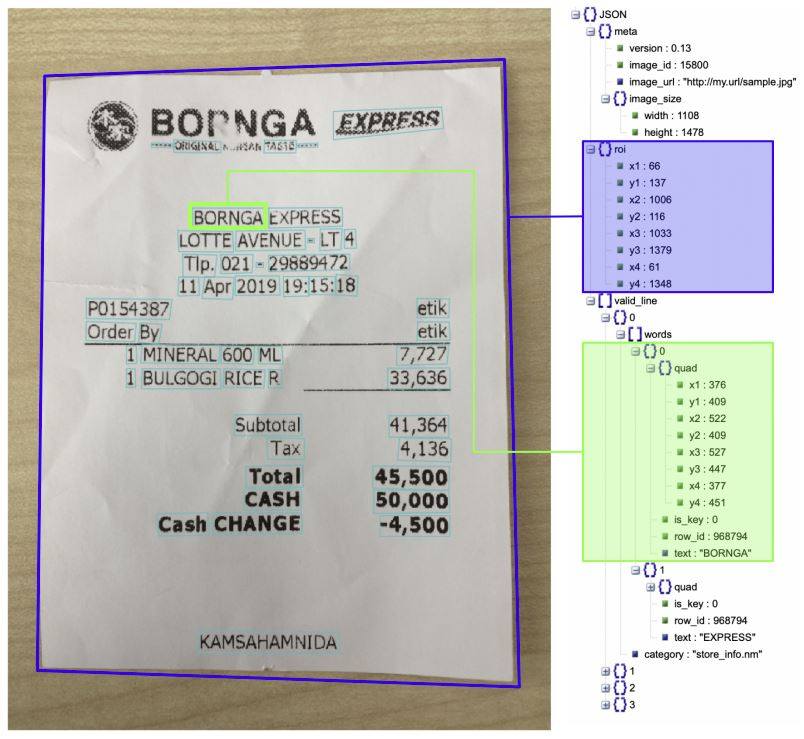
\includegraphics[width=0.6 \textwidth]{chapters/images/Methods/Datasets/CORD.JPG}
    \caption{ An example of receipt image (left) and json (right) \cite{park2019cord}}
    \label{fig:CORD_example_image}
\end{figure}

\begin{table}[!ht]
    \centering
    \begin{tabular}{lcccl}
    \hline
         No.& Superclass & \verb|#|Subclass & Proportion & Example  \\ \toprule
    % \hline
         1 & store info. & 9 & 0.134 & store name, address, telephone number \\
         2 & payment info. & 2 & 0.092 & visiting time, card company \\
         3 & menu & 16 & 0.510 & menu name, quantity, price, submenu \\
         4 & void menu & 6 & 0.0002 & menu name, quantity, price \\
         5 & subtotal & 8 & 0.073 & subtotal price, discount, service charge, tax\\
         6 & total & 8 & 0.145 & total price, amount of credit/debit card\\
         7 & void total & 4 & 0.00015 & void total, void tax\\
         8 & etc. & 1 & 0.045 & table number, membership points \\
         \hline
         Total & &54&1.0 & \\ \bottomrule
    \end{tabular}
    \caption{CORD\cite{park2019cord} statistics}
    \label{tab:CORD_statistics}
\end{table}


\begin{table}[!ht]
    \centering
    \captionsetup{justification=centering}
    \begin{tabular}{lccl}
    \hline
        \textbf{model} & \textbf{Precision} & \textbf{Recall} & \textbf{F1}  \\ \toprule
         
         LiLT\(\text{[EN-R]}_{BASE}\) &  0.959&  0.961& 0.960 \\
         LiLT\(\text{[InfoXLM]}_{BASE}\) & 0.957 & 0.958 & 0.957 \\ \bottomrule
    \end{tabular}
    \caption{Results of EN-R and InfoXLM with \acrshort{lilt} for \acrfull{ser} task on CORD \cite{park2019cord} dataset}
    \label{tab:cord_model_comparision}
\end{table}


\subsection{XFUND}

Datasets described in previous sections are monolingual. Multimodal pre-training using text, layout and images has achieved \acrshort{sota} perfomance. Therfore \cite{xfund} introduce a human-annotated multilingual form understanding benchmark dataset titled \textbf{XFUND}. Performing task such as template collection, form creation, key-value annotation and data finalization, spending around 1,500 hours of human labor, XFUND includes form understanding samples in total 7 languages (Chinese, Japanese, Spanish, French, Italian, German, Portuguese). In \Cref{fig:XFUND}, samples from dataset is shown, where red denotes the header, green indicates the keys and blue indicates the values. The statistics of the dataset is describe in \Cref{tab:XFUND_statistics}. A comperision of different models on \acrshort{ser} using XFUND is shown in \Cref{tab:Comparision_Xfund}.  

\begin{figure}[!ht]
    \begin{subfigure}{\textwidth}
    \centering
    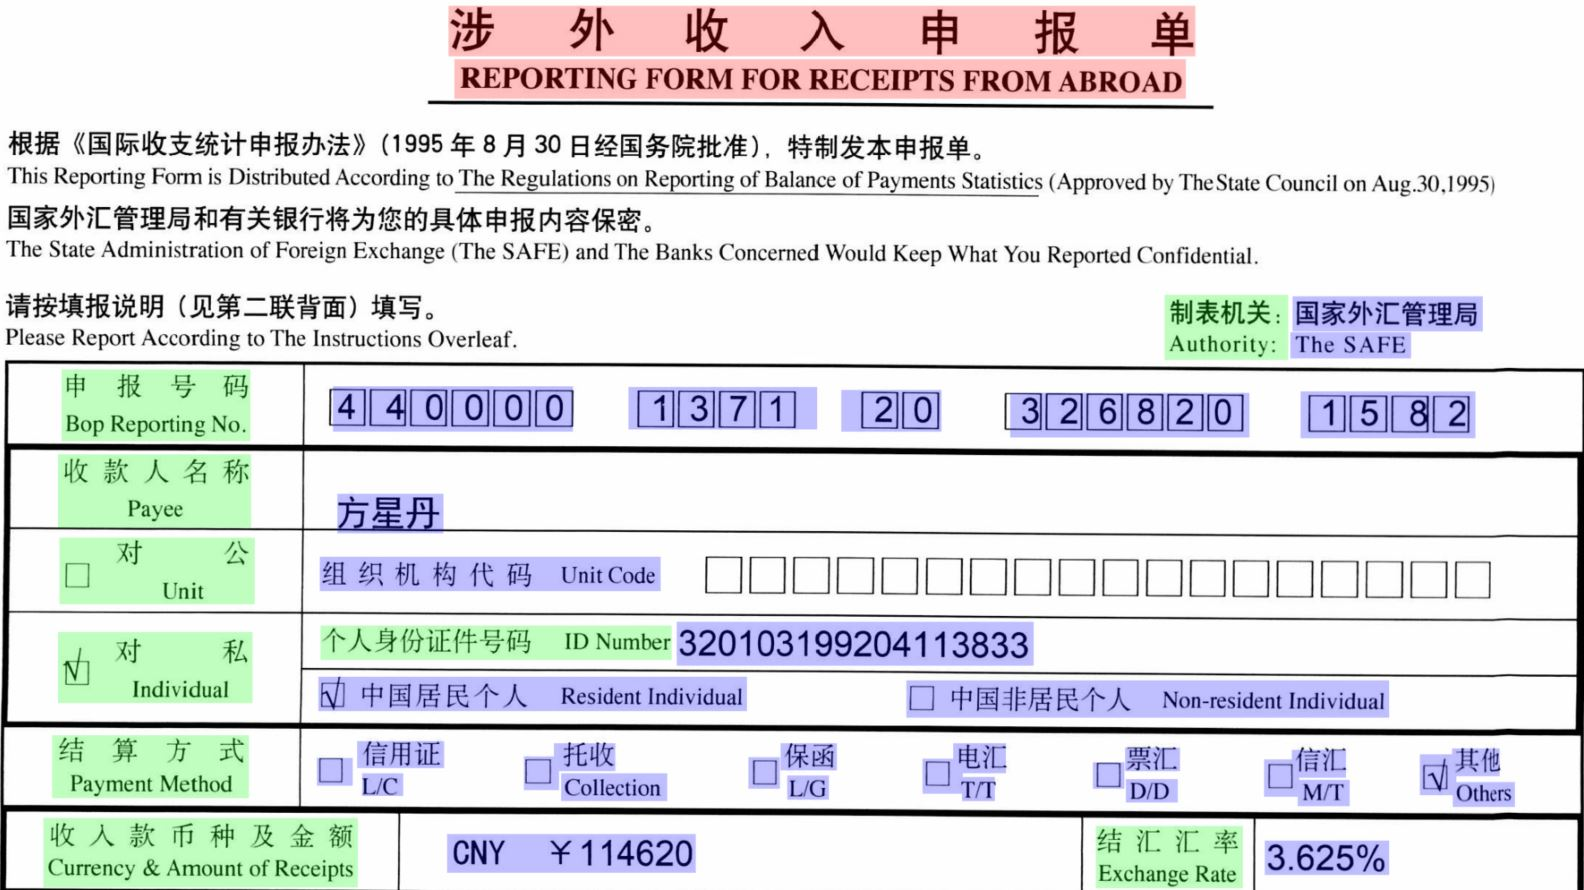
\includegraphics[scale=0.3]{chapters/images/Literature_review/LayoutXLM_Results_Chinese.JPG}
    \caption{Language: Chinese}
    \label{subfig_xfund:a}
    \end{subfigure}
    \begin{subfigure}{\textwidth}
    \centering
    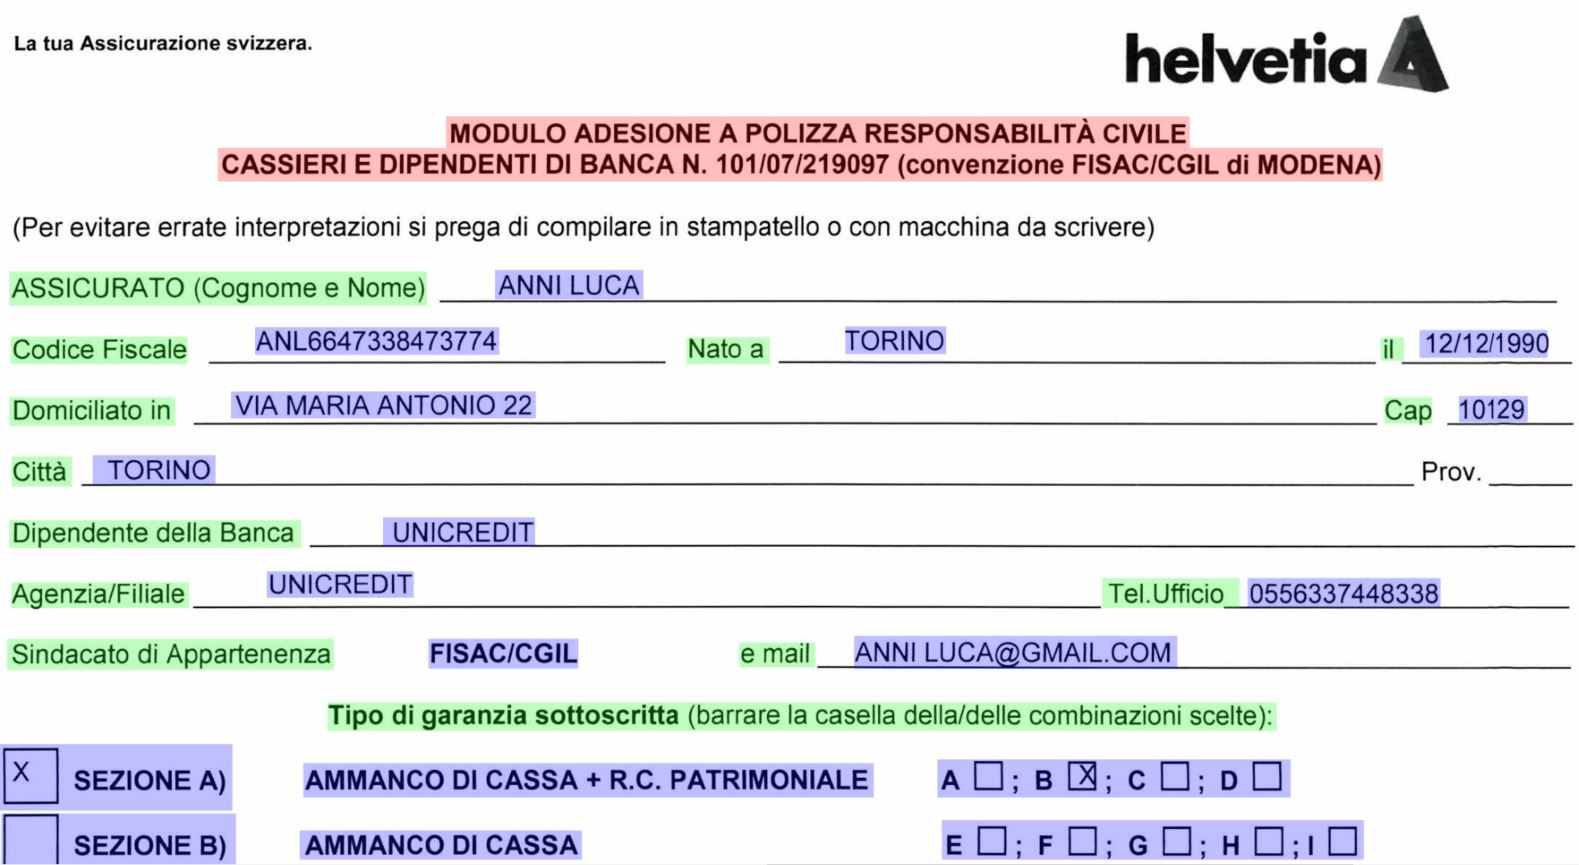
\includegraphics[scale=0.3]{chapters/images/Literature_review/LayoutXLM_Results_Italian.JPG}
    \caption{Language: Italian}
    \label{subfig_xfund:b}
    \end{subfigure}
    \caption{Classification results of LayoutXLM in two different language \cite{xu2021layoutxlm}}\label{fig:XFUND}
\end{figure}

% Please add the following required packages to your document preamble:
% \usepackage{booktabs}
% \usepackage{multirow}
\begin{table}[H]
\centering
\begin{tabular}{@{}lllllll@{}}
\hline
                 \textbf{Lang} & \textbf{Split}  &\textbf{Header}  &\textbf{Question}  & \textbf{Answer}  &\textbf{Other}  &\textbf{Total}  \\ \toprule
\multirow{2}{*}{ZH} &  training&229  &  3,692& 4,641  & 1,666  &10,228  \\ 
                  &  testing& 58  &1,253  & 1,732  & 586  & 3,629  \\ \midrule
\multirow{2}{*}{JA} & training & 150  & 2,379  & 3,836  & 2,640  & 9,005  \\
                  &  testing & 58  & 723  & 1,280  & 1,322  & 3,383  \\\midrule
\multirow{2}{*}{ES} & training  &  253& 3,013  & 4,254  &3,929  &11,449  \\
                  &  testing&  90& 909 &1,218  &1,196  &3,413  \\\midrule
\multirow{2}{*}{FR} & training & 183  &2,497  &3,427  &2,709  &8,816  \\
                  &  testing&66  &1,023  &1,281  &1,131  &3,501  \\\midrule
\multirow{2}{*}{IT} &  training &166  &3,762  &4,932  &3,355  &12,215  \\
                  &  testing& 65 &1,230  &1,599  &1,135 &4,029  \\\midrule
\multirow{2}{*}{DE} &training  &155  &2,609  &3,992  &1,876  &8,632  \\
                  &  testing&59  &858  &1,322  &650  &2,889  \\\midrule
\multirow{2}{*}{PT} & training &185  & 3,510 &5,428  &2,531   &  11,654\\
                  &  testing &59  &1,288  &1,940  &882  &4,169 \\ \bottomrule
\end{tabular}
\caption{Statistics of the XFUND \cite{xfund}}
\label{tab:XFUND_statistics}
\end{table}

\begin{table}[!ht]
    \centering
    \begin{tabular}{lcccccccl}
    \toprule
          Model&ZH&JA&ES&FR&IT&DE&PT  \\ \midrule
         XLM-RoBERTa\(_{BASE}\)$^1$& 0.877&0.776&0.610&0.674&0.668&0.681&0.681 \\
         InfoXLM\(_{BASE}\)&  0.886 & 0.786 & 0.623 &0.701 & 0.675 & 0.706 & 0.700 \\
         LayoutXLM\(_{BASE}\) &  0.892 & 0.792 & 0.755 & 0.790 & 0.808 & 0.822 & 0.790 \\ \midrule
         LiLT[InfoXLM]\(_{BASE}\) &  0.893 & 0.796 & 0.791& 0.795& 0.837& 0.823& 0.822 \\ \bottomrule
    \end{tabular}
    \caption{Language-specific fine-tuning F1 for \acrshort{ser} task on XFUND. $^1$\cite{li2021cross}}
    \label{tab:Comparision_Xfund}
\end{table}


